
\section{Compiler Infrastructure}

Compilers are programming tools responsible for translating programs in a given source language to a lower-level target language.
This compilation process must preserve the program semantics.
Moreover, compilers are also expected to produce a good quality representation of the program in the target language, optimising for a given objective function.
An important objective function is code size, i.e., the optimisation goal is to produce a representation of the program as small as possible.

Compilers are usually organised in \textit{three-phases}, as shown in Figure~\ref{fig:3-phase-compiler}: frontend, optimiser, and backend.
The frontend is responsible for parsing, validating and diagnosing errors in the source code.
This parsed source code is then translated into an intermediate representation, which is the LLVM IR in this case.
The optimiser is responsible for doing a broad variety of transformations, that are usually independent of language and target machine, to improve the code's performance.
The backend, also known as the code generator, then translates the code from the intermediate representation onto the target instruction set.
It is common for the backend to also perform some low-level optimisations that take advantage of unusual features of the supported architecture.
%Common parts of a compiler backend include instruction selection, register allocation, and instruction scheduling.

\begin{figure}[h]
  \centering
  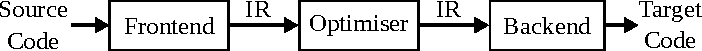
\includegraphics[scale=0.9]{src/background/figs/3-phase-compiler.pdf}
  \caption{Overview of the three-phase compiler infrastructure.}
  \label{fig:3-phase-compiler}
\end{figure}

However, these \textit{three-phases} represent only a simplified view of their designed.
In order to manage the complexity involved in optimising compilers, modern compilers are usually designed in a highly modular manner, where they are organised as a series of phases that sequentially analyse and transform the program being compiled.
For example, the frontend is subdivided into multiple phases.
The \textit{lexer} is responsible for tokenising the input stream of characters from the source code.
This token stream is then consumed by the \textit{parser}, producing a language-specific \textit{Abstract Syntax Tree} (AST).
The AST is an intermediate representation used during the semantic analysis, before being lowered to another intermediate representation.

\begin{figure}[h]
  \centering
  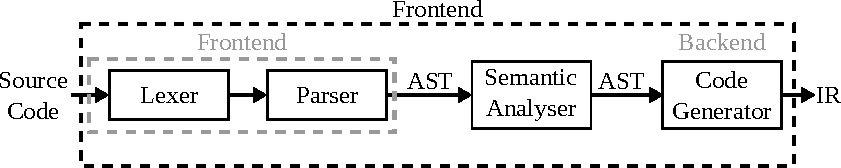
\includegraphics[scale=0.9]{src/background/figs/compiler-frontend.pdf}
  \caption{Breakdown of the frontend, illustrating how compilers are organised as a series of phases.}
  \label{fig:compiler-frontend}
\end{figure}

\begin{figure}[h]
\centering
\begin{subfigure}{\textwidth}
\centering
  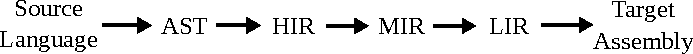
\includegraphics[scale=0.9]{src/background/figs/ir-lowering-sequence.pdf}
  \caption{An overview of representations and their level of abstractions used during the compilation pipeline.}
  \label{fig:ir-lowering-sequence-general}
\end{subfigure}
\begin{subfigure}{\textwidth}
\centering
  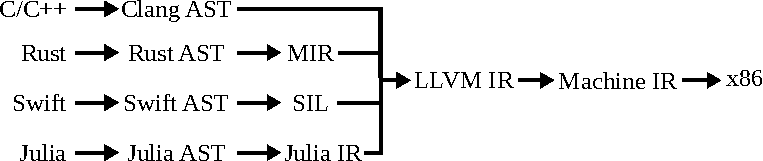
\includegraphics[scale=0.9]{src/background/figs/ir-lowering-sequence-example.pdf}
  \caption{An example of the sequence of representations used in real compilers for different programming languages.}
  \label{fig:ir-lowering-sequence-example}
\end{subfigure}
\caption{Sequence of representations used during the compilation pipeline in modern compilers.}
\label{fig:ir-lowering-sequence}
\end{figure}

Several intermediate representations, with different levels of abstraction, are used during this compilation process from the source to the target language.
Different analyses and optimisations are better modelled at different abstraction levels.
Figure~\ref{fig:ir-lowering-sequence-general} illustrates the sequence of representations used by modern compilers, each one having a progressively lower level than the previous one.
The source language is parsed into an AST, which is then commonly lowered to a high-level intermediate representation (HIR).
As shown in Figure~{fig:ir-lowering-sequence-example}, this HIR is usually a language-specific IR, such as the Swift Intermediate Language (SIL), which is used to solve domain-specific problems~\cite{lattner20}.
A popular mid-level intermediate representation (MIR) is the LLVM IR, which is shared among many compilers.
In the LLVM compiler infrastructure, the LLVM IR is lowered into a low-level representation (LIR), called the Machine IR, which is then lowered into the target assembly language.
This final process might actually involve multiple intermediate representations depending on the backend being used.


\subsection{Link-Time Optimisations}
%% benefits of LTO
%% challenges with LTO
%% mention partial LTO, such as ThinLTO

Figure~\ref{fig:full-pipeline} illustrates the standard pipeline for the compilation of multiple source files.
Compilers normally operate on a single translation unit at a time, where a translation unit includes a single source file and its expanded headers.
Each translation unit is optimised separately and compiled into a single native object file.
Finally, the linker combines multiple object files into a resulting binary or library.

\begin{figure}[h]
  \centering
  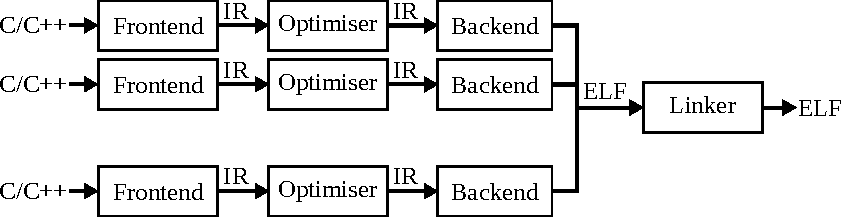
\includegraphics[scale=0.85]{src/background/figs/full-pipeline.pdf}
  \caption{Overview of the three-phase compiler infrastructure.}
  \label{fig:full-pipeline}
\end{figure}

However, this approach limits the impact of inter-procedural optimisations (IPO) to within each individual translation unit.
For example, if we have two identical functions defined in different translation units, they will not be merged using the approach shown in Figure~\ref{fig:full-pipeline}.
In order to achieve larger benefits from IPO, the optimisation scope can be increased to include multiple translation units.
When the scope includes all translation units being linked into an executable, the compiler can perform  more aggressive optimisations that rely on whole-program information~\cite{johnson17}.

\begin{figure}[h]
  \centering
  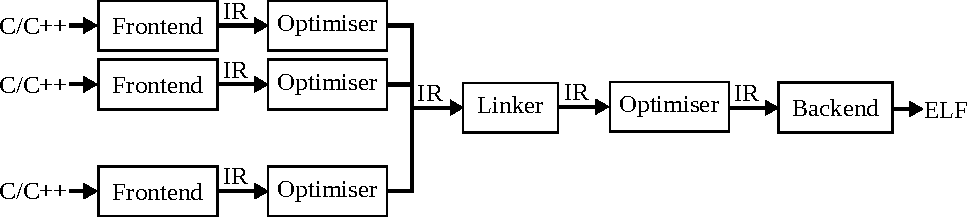
\includegraphics[scale=0.85]{src/background/figs/full-pipeline-LTO.pdf}
  \caption{Overview of the three-phase compiler infrastructure.}
  \label{fig:full-LTO-pipeline}
\end{figure}

Figure~\ref{fig:full-LTO-pipeline} illustrates a common mechanism for enabling whole-program optimisation called link-time optimisation (LTO).
In this approach, optimisations are applied in two different moments.
First, we have \textit{early} optimisations being applied on a per translation unit basis.
However, we also have \textit{late} optimisations being applied after all translation units are linked together.
Therefore, allowing important inter-procedural optimisations to be applied on the whole-program, across translation units.

In the LTO mode, compilers delay the generation of native object files.
As shown in Figure~\ref{fig:full-LTO-pipeline}, all translation units are linked while still in an IR better suited for the late optimisations.
